\section{Method}
\label{chahawk:sec:method}

In the following, we describe the architecture and methodology of HAWK. We explain our approach by using the following running example:
\texttt{Which recipients of the Victoria Cross died in the Battle of Arnhem?}
While this question cannot be answered by using solely DBpedia or Wikipedia abstracts, combining knowledge from DBpedia and Wikipedia abstracts allows deriving an answer to this question. More specifically, DBpedia allows to retrieve all recipients of the Victoria Cross using the triple pattern \texttt{?uri dbo:award dbr:Victoria\_Cross.}

In order to find out whether the returned resources died in the Battle of Arnhem, the free text abstract of those resources need to be checked. For example, the abstract for John Hollington Grayburn contains the following information: 
`he went into action in the Battle of Arnhem [...] but was killed after standing up in full view of a German tank'.

Figure~\ref{chahawk:fig:architecture} gives an overview of the architecture of HAWK. In the following we describe the depicted steps in more detail.%: POS-tagging, entity annotation, dependency parsing, linguistic pruning, semantic annotation, SPARQL query generation, pruning and ranking.

\begin{figure}
\centering
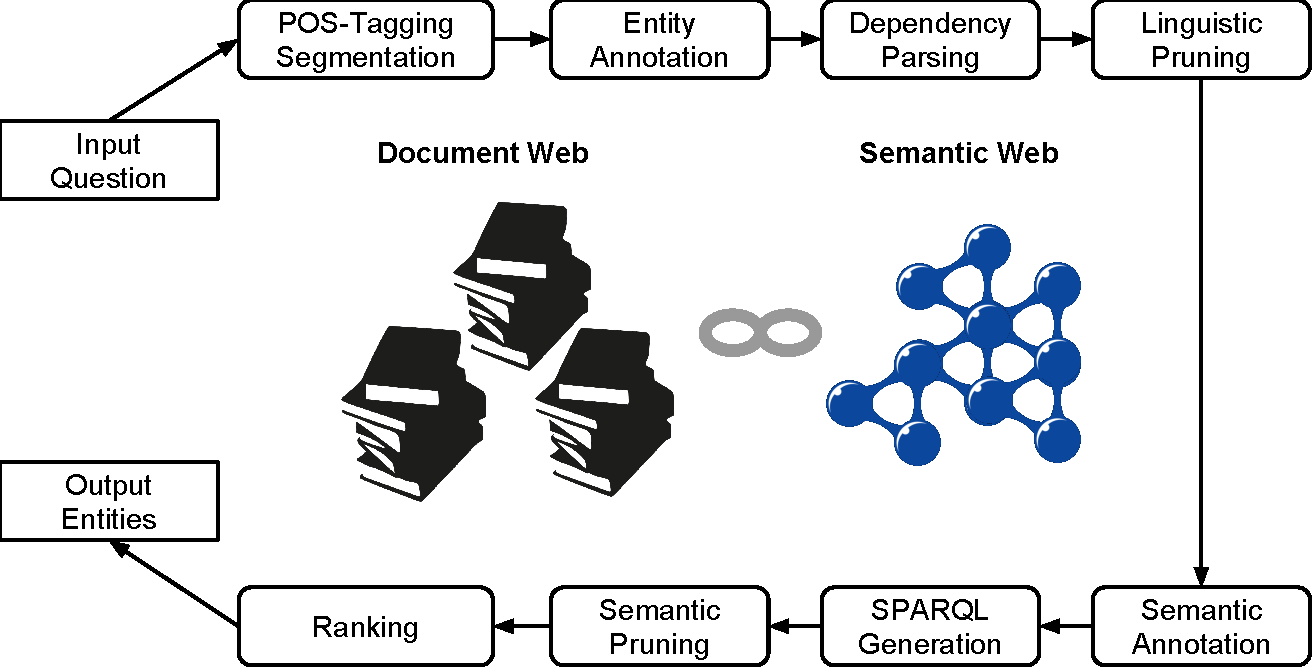
\includegraphics[width=0.8\linewidth]{chapter_four/ESWC_HAWK/HAWK_architecture}
\caption{Architectural overview of HAWK.}
\label{chahawk:fig:architecture}
\end{figure}


\subsection{POS-Tagging, Segmentation}
%\todo[inline]{re is no tokenisation/segmentation component in the pipeline?}
A large number of frameworks have been developed for these purposes over the last years. 
We rely on \emph{clearNLP}~\cite{choi2011getting} which is based on transition-based dependency parsing and sophisticated segmentation algorithm.
Regarding our running example the following POS-tags are generated:
\texttt{Which(WDT) recipients(NNS) of(IN) the(DT) Victoria(NNP) Cross(NNP) died(VBN) in(IN) the(DT) Battle(NNP) of(IN) Arnhem(NNP)?(PUNCT)}

\subsection{Entity Annotation}
HAWK identifies named entities and tries to link them to semantic entities from the underlying knowledge base, in our case DBpedia 3.9, via well-established entity annotation tools, also called entity tagging tools:
\begin{itemize}
\item \textbf{Wikipedia Miner}~\cite{milne2008learning} is based on different facts like prior probabilities, context relatedness and quality, which are then combined and tuned using a classifier.
\item \textbf{DBpedia Spotlight}~\cite{spotlight} %, one of the first semantic entity annotation approaches, 
was published in 2011. 
This tool combines named entity recognition and disambiguation based on DBpedia.
\item \textbf{TagMe 2}~\cite{TagMe2} is based on a directory of links, pages and an inlink graph from Wikipedia.
The approach recognizes entities by matching terms with Wikipedia link texts and disambiguates the match using the in-link graph and the page dataset.
%Afterwards, TagMe 2 prunes identified named entities which are considered as non-coherent to the rest of the named entities in the input text.  
\item \textbf{FOX}~\cite{FOX} has been introduced 2014 as an ensemble learning-based approach combining several state-of-the-art named entity recognition approaches. 
The FOX framework outperforms the current state of the art entity recognizers and relies on the entity linking tool AGDISTIS~\cite{agdistis_iswc}.
\end{itemize}
Additionally, we implemented two artificial spotters for evaluation:
\begin{itemize}
\item \textbf{Union} is a spotter that combines the result sets of the above introduced spotters and returns thus a superset of all spotters.
\item \textbf{Optimal} will spot all entities from the gold standard to be able to ignore spotting influences in the following steps of the pipeline.
\end{itemize}

For our running example, an optimal spotter identifies \texttt{Victoria\_Cross} and \texttt{Battle\_of\_Arnhem} as resources form DBpedia.
HAWK annotates the POS-tag \texttt{ADD} to it. % for our running example from above.
The influence of the entity annotation module is evaluated in Section~\ref{chahawk:sec:evaluation}.

\subsection{Dependency Parsing}
HAWK performs noun phrase detection for semantically meaningful word groups not yet recognized by the entity annotation system also known as chunking.
This detection reuses the above mentioned POS-tagger. % based on a-priori part-of-speech (POS) tagging~\cite{choi2011getting}.
Input tokens will be combined following manually-crafted linguistic heuristics derived from the benchmark questions, and their POS-tag is changed to \texttt{CNN}.
Thus, the input is a natural language question (list of keywords) and the output is a list of chunks, see Algorithm~1.
HAWK's modular structure allows for an easy exchange of the POS-tagger or dependency parser.

\begin{algorithm}[H]
\SetAlgoLined
\KwData{Tokenized question ($list$) with Part-of-Speech-tags (POS-tags)}
	subsequence = ()\;
	\For{$t \in [0,|list|]$ }{
			token = list.get($t$)\;
			%// look for start "RB|JJ|NN(.)*"
			\eIf{$subsequence = \emptyset$}{
			    \lIf{$pos(t) \in (\mathrm{CD|JJ|NN(.)^*|RB(.)^*})$} {
				subsequence.add(token)
				}
			}
			%// split "of the" or "of all" via pos\_i=IN and pos\_i+1=DT
			{
    			\uIf{$t + 1 < |list| \wedge pos(t) \in (\mathrm{IN}) \wedge pos(t+1) \in (\mathrm{(W)?DT})$} {
    				\lIf{$subsequence.size() >= 2$} {
    					combine(subsequence)
    				}
    		        subsequence = ()\;
    			}
    		%	// do not combine NNS and NNPS but combine "stage name", "British Prime minister"
    			\uElseIf{$pos(t - 1) \in (\mathrm{NNS}) \wedge pos(t) \in (\mathrm{NNP(S)?})$} {
    			    \lIf{$subsequence.size() > 2$} {
    					combine(subsequence)
    				}
    		        subsequence = ()\;
    			}
    		%	// finish via VB* or IN -> null or IN -> DT or WDT (now a that or which follows)
    			\uElseIf{$!pos(t - 1) \in (\mathrm{JJ|HYPH}) \wedge (pos(t) \in (\mathrm{VB|WDT|IN})))$} {
    		%		// more than one token, so summarizing makes sense
    			    \lIf{$subsequence.size() > 1$} {
    					combine(subsequence)
    				}
    		        subsequence = ()\;
    			}
    		    \uElseIf{$pos(t) \in (\mathrm{NN(.)^*|RB|CD|CC|JJ|DT|IN|PRP|HYPH|VBN})$} {
    				subsequence.add(token)
    			}
    			\uElse{
    		        subsequence = ()\;
    			}
    		}
        }
\caption{Algorithm for combining noun phrases}
\end{algorithm}
\label{listing:nouncombiner}


Subsequently, in order to capture linguistic and semantic relations, HAWK parses the query using dependency parsing and semantic role labeling~\cite{choi2011getting}.
The dependency parser is given the chunked question. 
The generated pre\-dicate-argument tree is directed, acyclic, and all its nodes contain their POS-tags as well as their labels, see Figure~\ref{chahawk:fig:dependency_tree}.


\subsection{Linguistic Pruning}

The natural language input can contain tokens that are meaningless for retrieving the target information or even introduce noise in the process.
HAWK therefore prunes nodes from the predicate-argument tree based on their POS-tags, e.g., deleting all \texttt{DET} nodes, interrogative phrases such as \texttt{Give me} or \texttt{List}, and auxiliary tokens such as \texttt{did}.
Algorithm~2 details the algorithm for removing nodes.
Figure~\ref{chahawk:fig:prunedtree} depicts the predicate-argument tree obtained for our running example after pruning.% of unnecessary nodes.

\begin{algorithm}[H]
\SetAlgoLined
\KwData{Dependency-argument tree with Part-of-Speech-tags}
Queue queue = [tree.getRoot()]\;
\While{$queue != \emptyset$} {
	node = queue.poll()\;
    \If{$pos(node) \in (\mathrm{WDT|POS|WP\$|PRP\$|RB|PRP|DT|IN|PDT})$} {
	tree.remove(node)\;
}
	queue.add(node.getChildren())\;
}
\If{$root.label == ("Give")$} {
	\For{$childNode \in root.getChildren()$} {
		\lIf{$childNode == "me"$} {
			tree.remove(childNode)
		}
	}
}
\lIf{root.label $\in\{ "List", "Give"\}$}{
	tree.remove(root)
}
\caption{Algorithm for pruning noisy nodes}
\end{algorithm}
\label{listing:lingpruning}


\begin{minipage}{0.57\textwidth} 
\centering
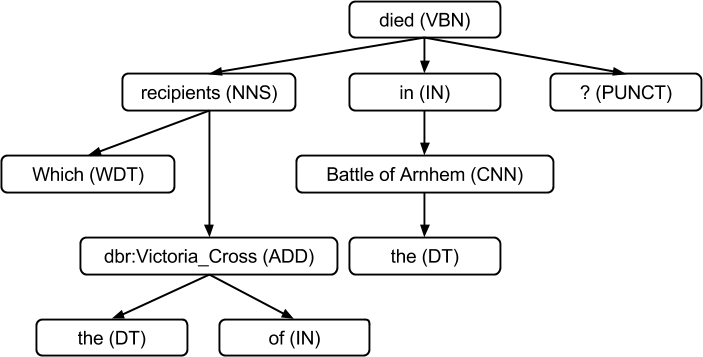
\includegraphics[width=\linewidth]{chapter_four/ESWC_HAWK/hawk_tree_full}
\captionof{figure}{Predicate-argument tree for the example question `Which recipients of the Victoria Cross died in the Battle of Arnhem?'}
\label{chahawk:fig:dependency_tree}
\end{minipage}
\hfill
\begin{minipage}{0.36\textwidth}
\centering
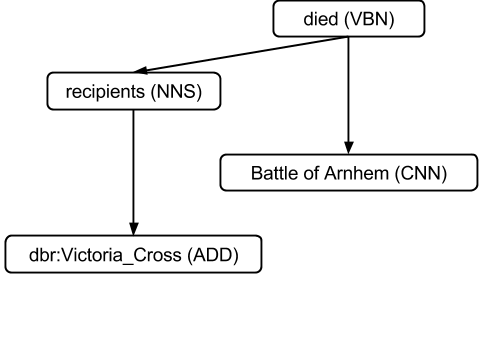
\includegraphics[width=\linewidth]{chapter_four/ESWC_HAWK/hawk_tree_pruned}
\captionof{figure}{Tree after pruning. Argument edges are ordered from left to right.}
\label{chahawk:fig:prunedtree}
\end{minipage}

\subsection{Semantic Annotation}
After linguistic pruning, HAWK annotates each node in the tree with possible concepts from the knowledge base and its underlying ontology.
To this end, our framework uses information about possible verbalizations of ontology concepts, based on both \texttt{rdfs:label} information from the ontology itself and (if available) verbalization information contained in lexica.
%lexiconexisting manually crafted English lexicon\footnote{\url{https://github.com/cunger/lemon.dbpedia}} for DBpedia. 
% we generated triples of the form $\langle$\emph{reference},\,\texttt{rdfs:label},\,\texttt{"}\emph{form}\texttt{"}$\rangle$, that link an ontology element (\emph{reference}) to its written representation (\emph{form}) in the lexicon. 
In general, such lexica offer a range of lexical variants beyond the labels present in DBpedia. For example, for the property \texttt{spouse}, the DBpedia English lexicon\footnote{\url{https://github.com/cunger/lemon.dbpedia}} provides the noun entries `wife' and `husband' as well as the verb entry `to marry'.
%, 
%resulting in the following triples:

%\begin{itemize}
%\item \texttt{http://dbpedia.org/ontology/spouse rdfs:label "wife" .}
%\item \texttt{http://dbpedia.org/ontology/spouse rdfs:label "husband" .}
%\item \texttt{http://dbpedia.org/ontology/spouse rdfs:label "marry" .}
%\end{itemize}

HAWK now tries to match each node label to a class or property from the DBpedia ontology using fuzzy string matching.
%with an edit distance of 1 as provided by the Lucene framework\footnote{\url{http://lucene.apache.org/}}.
Moreover, HAWK follows intuitions used in~\cite{tbsl} to lower the number of annotations avoiding additional computational effort. 
In particular, we consider the POS-tag of nodes to determine the type of the target reference:
\begin{itemize}
\item nouns correspond to object type properties and classes
\item verbs correspond to object type properties
\item question words (e.g., \texttt{who} or \texttt{where}) correspond to classes (e.g., \texttt{Person} or \texttt{Place})
\end{itemize}

Afterwards, HAWK ranks properties according to their prominence score in the knowledge base and returns only the top n properties.
If the search does not retrieve any annotations, we additionally ask the lemmata of the node label and repeat the above described process to increase recall.

Considering our running example,the nodes \texttt{died (VB)} will be annotated with \texttt{dbo:deathplace} and \texttt{dbo:deathdate} and the node \texttt{recipients (NNS)} with \texttt{dbo:award}.
After this step, either a node is annotated with a reference from the knowledge base % it is a disambiguated resource 
or it will be lead to a full-text lookup to be resolved to a knowledge base resource as explained in the following section.

%\begin{table}[htb]
%\caption{Annotations of nodes from running example.}
%\centering
%    \begin{tabular}{ll}
%        \toprule
%             & \textbf{Annotation}\\
%        \midrule
%            died& \texttt{dbo:deathplace}, \texttt{dbo:deathdate} \\
%            recipients & \texttt{dbo:award} \\
%        \bottomrule
%    \end{tabular}
%\label{tab:annotations}
%\end{table}

\subsection{Generating SPARQL Queries}
\label{chahawk:sec:full-text}

The core of HAWK is the generation of SPARQL queries from annotated and pruned predicate-argument trees.
%\todo[inline]{The indexed properties used for  text searches will be described in Section 2.6. }
It uses an Apache Jena FUSEKI\footnote{\url{http://jena.apache.org/documentation/serving_data/}} server, which implements the full-text search predicate \texttt{text:query} on a-priori defined literals over configured predicates. % using the Lucene search query syntax. 
Especially, the following predicates were indexed as they yield a high information content with respect to DBpedia 3.9:
\begin{itemize}
 \item \texttt{dbpedia:abstract} for general interest information about a resource not modelled appropriately in the knowledge base
 \item \texttt{rdfs:label} to match resources not found by the entity annotation system%, e.g., \url{http://dbpedia.org/resource/The\_Crown}
 \item \texttt{dbpedia:redirect} to identify common synonyms, e.g., `first man in space' pointing to \url{http://dbpedia.org/resource/Yuri_Gagarin}
 \item \texttt{dc:subject} for linking top-level categories like `assassin' to resources like \url{http://dbpedia.org/resource/James_Earl_Ray}
\end{itemize}
Currently, HAWK resolves full-text information either by using exact matches of node labels or fuzzy matches on each non-stopword token of a label; Table~\ref{tab:exact_fuzzy} depicts the two possibilities for the running example.

\begin{table}[htb!]
\centering
\caption{Examples for full-text query types.}
\begin{tabular}{l@{\quad}l@{\quad}l}
\toprule
\textbf{Query Type} & \textbf{Query Syntax} & \textbf{Node label}\\
\midrule
Exact & \texttt{?var text:query ('Battle of Arnhem')}  & Battle of Arnhem\\
Fuzzy & \texttt{?var text:query ('Battle\textasciitilde1 AND Arnhem\textasciitilde 1')} & Battle of Arnhem\\
\bottomrule
\end{tabular}
\label{tab:exact_fuzzy}
\end{table}
To capture the full semantics of an input question, HAWK traverses the predicated-argument tree in a pre-order walk to reflect the empirical observation that i) related information are situated close to each other in the tree and ii) information are more restrictive from left to right.
This breadth-first search visits each node and generates several \emph{possible triple patterns} based on the number of annotations and the POS-tag itself. 
That is, for each node a set of SPARQL query patterns is generated following the rules depicted in Table~\ref{tab:triple_patterns} w.r.t. ontology type information, e.g., a variable bound to the class \texttt{Place} will not have an outgoing predicate \texttt{birthPlace}.

Using this approach allows HAWK to be independent of SPARQL templates %, such as used by TBSL~\cite{tbsl}, 
and to work on natural language input of any length and complexity.
Each pattern contains at least one variable from a pre-defined set of variables, i.e., \texttt{?proj} for the resource projection variable, \texttt{?const} for resources covering constraints related to the projection variable as well as a variety of variables for predicates to inspect the surrounding of elements in the knowledge base graph. 
Table~\ref{tab:triple_patterns_example} shows generated triple patterns for parts of the example query.
\begin{table}[htb!]
\centering
\caption{Generated triple patterns for running example.}
\begin{tabular}{l@{\quad}l}
\toprule
\textbf{Node Type} & \textbf{Query Fragment} \\
\midrule
\multirow{2}{*}{CNN} & \texttt{?proj text:query ('Battle of Arnhem')} \\
& \texttt{?const text:query ('Battle of Arnhem')} \\
%& \texttt{?proj text:query ('Battle~1 AND Arnhem~1')} \\
%& \texttt{?const text:query ('Battle~1 AND Arnhem~1')}\\
\midrule
\multirow{2}{*}{Verb} & \texttt{?proj dbo:deathPlace ?const} \\
 & \texttt{?const dbo:deathPlace ?proj} \\
\bottomrule
\end{tabular}

\label{tab:triple_patterns_example}
\end{table}

\begin{table}[htb!]
\centering
\caption{Triple patterns for generating SPARQL queries while traversal.}
\begin{tabular}{ll}
\toprule
\textbf{Node POS-tag and non-empty annotations} & \textbf{Query Fragment} \\
\midrule
VB(.)* & \texttt{?proj Annotation ?const.} \\
VB(.)* & \texttt{?const Annotation ?proj.} \\
VB(.)* & \texttt{?const ?proot ?proj.} \\
NN(.)*$|$WRB & \texttt{?proj  Annotation ?const.} \\
NN(.)*$|$WRB & \texttt{?const Annotation ?proj.} \\
NN(.)*$|$WRB & \texttt{?proj a Annotation.} \\
NN(.)*$|$WRB & \texttt{?const a Annotation.} \\
NN(.)*$|$WRB & \texttt{?const text:query (node label)} \\
WP& \texttt{?const a Annotation.} \\
WP& \texttt{?proj a Annotation.} \\
%WP$|$NN(.)*$|$WRB& ignore \\
in all cases & add empty triple pattern\\
\midrule
\textbf{Node POS-tag and empty annotations} & \textbf{Query Fragment} \\
\midrule
CNN$|$NNP(.)*$|$JJ$|$CD&  \texttt{?proj text:query (node label)} \\
CNN$|$NNP(.)*$|$JJ$|$CD&\texttt{?const text:query (node label)} \\
VB(.)*& \texttt{?proj text:query (node label)} \\
VB(.)*&\texttt{?const text:query (node label)} \\
ADD& \texttt{?proj ?pbridge nodeURI.} \\
ADD& \texttt{FILTER (?proj IN (nodeURI))} \\
ADD&  \texttt{?proj text:query (node label)} \\
ADD& \texttt{?const text:query (node label)} \\
NN$|$NNS& \texttt{?proj text:query (node label)} \\
NN$|$NNS& \texttt{?const text:query (node label)} \\
%NN(.)*$|$WP$|$ADD$|$VB(.)*$|$CombinedNN$|$JJ$|$CD& ignore node \\
in all cases & add empty triple pattern \\
\bottomrule
\end{tabular}

\label{tab:triple_patterns}
\end{table}

During this process, each iteration of the traversal appends the generated patterns to each of the already existing SPARQL queries. 
This combinatorial effort results in covering every possible SPARQL graph pattern given the predicate-argument tree.



\subsection{Semantic Pruning of SPARQL Queries}

Producing the n-fold-cross-product of possible pattern combinations generates a huge number of SPARQL queries, most of which are semantically senseless,e.g., a city that has a birth date. 
To effectively handle this large set of queries and reduce the computational effort, HAWK implements various methods for pruning:
\begin{itemize}
\item \textbf{\#textfilter: } HAWK can safely assume that SPARQL queries containing full-text lookups over more than one variable or containing more than two node labels do not yield semantically senseful information and thus discards such queries. 
\item \textbf{\#unbound triple pattern}: SPARQL queries containing more than one triple pattern of the form \texttt{?varx ?vary ?varz} or one such triple pattern and only text searches, lead to a traversal of large parts of the knowledge base graph and high computational effort.
\item \textbf{Unconnected query graph: } SPARQL query graphs which are not connected from cartesian products are pruned for the sake of runtime and their lack of semantics.
\item \textbf{Cyclic triple: } Queries containing edges of the form \texttt{?s <http://xyz>  ?o. ?o <http://xyz> ?s} or \texttt{?s <http://xyz>  ?o. ?s <http://abc> ?o} are also removed. 
\item \textbf{Missing projection variable: } The before mentioned traversal and SPARQL generation process can produce SPARQL queries without triple patterns containing the projection variable. These queries are also removed from the set of queries.
\item \textbf{Disjointness: }
Also SPARQL queries with triple patterns violating disjointness statements are discarded:
\begin{itemize}
\item \texttt{?s a  cls . ?s p ?o .} if \texttt{cls} and domain of \texttt{p} are disjoint
\item \texttt{?o a  cls . ?s p ?o .} if \texttt{cls} and range of \texttt{p} are disjoint
\item \texttt{?s p1  ?o1 . ?s p2 ?o2 .} if domain of \texttt{p1} and \texttt{p2} are disjoint
\item \texttt{?s1 p1  ?o . ?s2 p2 ?o .} if range of \texttt{p1} and \texttt{p2} are disjoint
\item \texttt{?s p1  ?o . ?s p2 ?o .} if \texttt{p1} and \texttt{p2} are disjoint
\end{itemize}
Due to lack of explicit disjointness statements in many knowledge bases, we (heuristically) assume that classes and properties that are not related via subsumption hierarchy are disjoint.
%\item \textbf{Entity type mismatch: }\todo[inline]{Eigentlich sollte das ja schon beim entity lookup passieren, d.h. es macht Sinn für predicate auch nur in der Menge der properties zu suchen, dasselbe gilt für Klassen. eher ungünstig das hier überhaupt zu erwähnen, lässt unseren lookup nicht sehr schlau aussehen, und ist auch trivial.}
\end{itemize}

Although semantic pruning drastically reduces the amount of queries, it often does not result in only one query. HAWK thus requires a final ranking step before sending the SPARQL query to the target triple store.

\subsection{Ranking}
%\todo[inline]{motivate features more}
HAWK ranks queries using supervised training based on the gold standard answer set from the QALD-4 benchmark.
In the \emph{training phase}, all generated queries are run against the underlying SPARQL endpoint. 
Comparing the results to the gold standard answer set, HAWK stores all queries resulting with the same high F-measure.
Afterwards the stored queries are used to calculate an average feature vector comprising simple features mimicking a centroid-based cosine ranking.
HAWK's ranking calculation comprises the following components:
\begin{itemize}
\item \textbf{NR\_OF\_TERMS} calculates the number of nodes used to form the full-text query part as described in Section~\ref{chahawk:sec:full-text}.
\item \textbf{NR\_OF\_CONSTRAINTS} counts the amount of triple patterns per SPARQL query.
\item \textbf{NR\_OF\_TYPES} sums the amount of patterns of the form \texttt{?var rdf:type cls}.
\item \textbf{PREDICATES} generates a vector containing an entry for each predicate used in the SPARQL query.
%\item \textbf{2path motifs containing a variable with a text:filter}
%\todo[inline]{Paste picture of motifs here}
\end{itemize}

While running the \emph{test phase} of HAWK, the cosine similarity between each SPARQL query using the above mentioned features and the average feature vector of training queries is calculated.
Moreover, HAWK determines the target cardinality $x$, i.e., \texttt{LIMIT x}, of each query using the indicated cardinality of the first seen POS-tag of the input query, e.g., the POS-tag \texttt{NNS} demands the plural while \texttt{NN} demands the singular case and thus leads to different \texttt{x}.
The performance of this ranking approach is evaluated in Section~\ref{chahawk:sec:evaluation}.
%\todo[inline]{Show two queries, their vectors and their score.}

%\subsection{Demo}
%\begin{itemize}
%\item test queries
%\item verbalisation
%\item feedback loop?
%\end{itemize}
